\documentclass[a4paper]{article}

\title{Rapport de stage}
\usepackage[utf8]{inputenc}
\usepackage[francais]{babel}
\usepackage{amsmath}
\usepackage{eufrak}
\usepackage{graphicx}
\usepackage{listings}
\usepackage{verbatim}
\usepackage{sagetex}
\usepackage{array,multirow,makecell}
\usepackage{amssymb}

\newtheorem{Rem}{Remarque}[subsection]
\newtheorem{Ex}{Exemple}[subsection]
\newtheorem{Def}{Définition}[section]
\newtheorem{Prop}[Def]{Proposition}
\newtheorem{Th}[Def]{Théorème}
\lstset{language=Python}
\usepackage{fancyhdr}
\pagestyle{fancy}
\begin{document}

\author{Quentin Honoré}
\date{}
\maketitle
\newpage
\tableofcontents
\newpage
\section*{Remerciements}
\newpage
\section*{Introduction}
\newpage
\section{Présentation du LaBRI}
\newpage
\section{Les plans projectifs finis}
\subsection{Définition}
Soit P un ensemble fini (appelé points) et D un sous ensemble des parties de P (appelé droites). \\
On dit que le couple (P,D) est un plan projectif fini si et seulement si: \\
$\cdot$ Par deux points distincts passe une unique droite. \\
$\cdot$ Deux droites distinctes se coupent en un unique point. \\
$\cdot$ Il existe un quadrilatère (4 points tels que pour chaque triplet, les 3 points ne sont pas alignés).

\begin{Rem}
  $\cdot$ Les 2 premières propositions sont symétriques. \\
  $\cdot$ Un plan projectif est une structure d'incidence (un ensemble de points et un ensemble de droites).
\end{Rem}
  
\begin{Ex}
  On va construire un plan projectif fini d'ordre 2 (3 points par droite, et 3 droites se coupent en chaque point). On construit d'abord un quadrilatère. Dans cette géométrie, deux droites qui n'ont pas de points en commun sont dites parallèles. Les diagonales, les deux droites horizontales et les deux verticales \vspace{1\baselineskip}sont donc parallèles.\\
  Pourtant il nous faut bien une intersection pour tout couple de droites. On définit alors les intersections dites ``à l'infini'', c'est l'idée de base de la géométrie projective. De la même manière que pour le point de fuite chez les peintres, on dit que deux droites parallèles s'intersectent à l'infini. Imaginez vous sur une route, les deux bordures sont bien parallèles mais en regardant au loin, nous avons l'impression que la route se rétrécit pour ne devenir\vspace{1\baselineskip} qu'un point.\\
La première propriété nous dit maintenant que pour chaque couple de points, on a une unique droite. Nous allons donc construire la ``droite à l'infini'' qui passe par les points à l'infini (comme l'horizon dans la vie courante).
\begin{center}
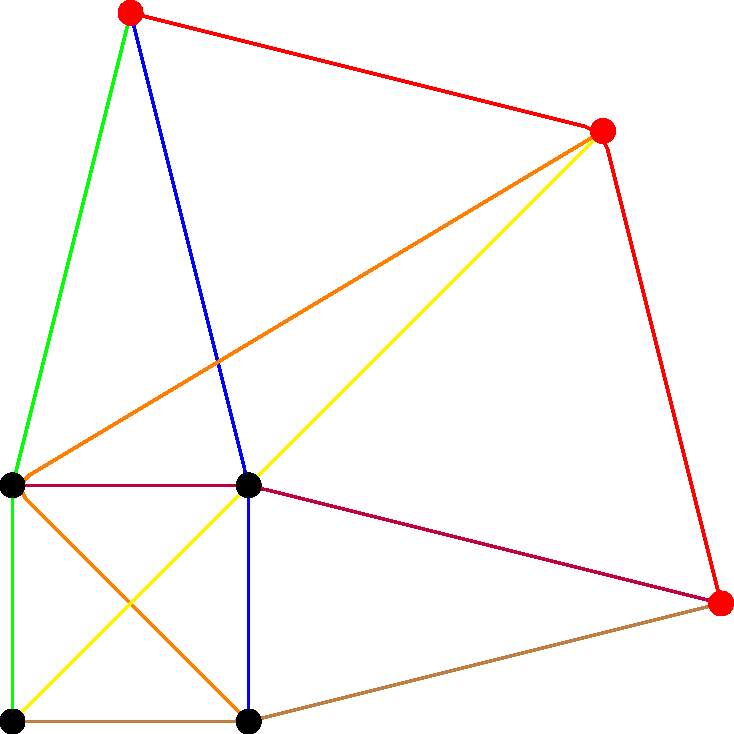
\includegraphics[scale=1.5]{test_tikz.pdf}
\end{center}
\vspace{2\baselineskip}
Les 3 propositions sont bien vérifiées.
\end{Ex}
\newpage
\begin{Ex}
  Le jeu du Dobble est un bon exemple de plan projectif fini. Si vous ne le connaissez pas, le Dobble est un jeu composé de 55 cartes sur lesquelles sont dessinés 8 objets\vspace{1\baselineskip} différents.\\
  A chaque tour, pour gagner, il faut reconnaître le plus rapidement quel est le symbole commun entre sa propre carte et celle au milieu. Le jeu ne serait alors pas juste si l'un-e des joueu-r-ses avait deux symboles en commun avec la carte du milieu tandis que l'autre n'en\vspace{1\baselineskip} a aucun. \\
 Ces cartes sont donc construites de telle manière que pour toute paire de carte, il y ait un et un seul objet en commun. On vérifie donc bien que si les cartes sont les droites et les symboles les points, alors pour deux droites distinctes, il y a un unique point d'intersection(ie. pour deux cartes, il y a un unique objet en comm\vspace{1\baselineskip}un).\\
 
\begin{center}
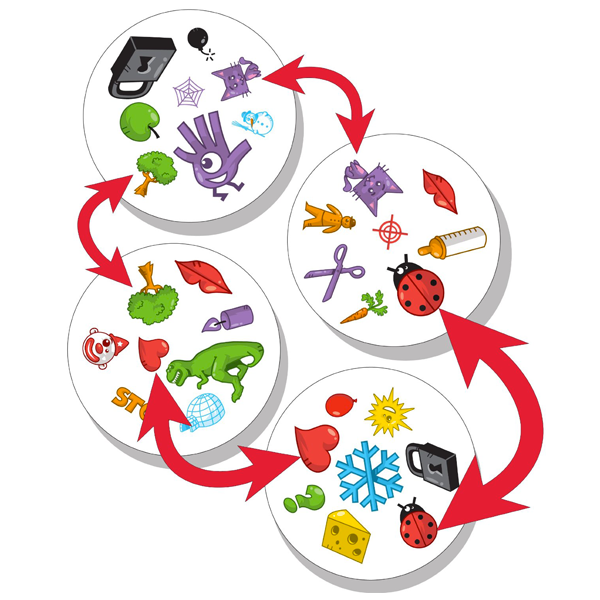
\includegraphics[scale=0.3]{dobble-2.jpg}
\end{center}
\end{Ex}
\begin{Prop}
Toutes les droites contiennent le même nombre de points. Par symétrie, par tout point passe le même nombre de droites. Soit k+1 ($k>=2$) ce nombre alors:
\begin{center}
$card(D)=card(P)=k^2+k+1$
\end{center}
\end{Prop}

\vspace{2\baselineskip}

En effet, si on considère un point P, k+1 droites passent par ce point. Sur chacune de ces droites, il y a k+1 points, donc k si on ne compte pas le point P. On a donc k(k+1) points en plus du point P, soit:
\begin{center}
$card(P)=k(k+1)+1=k^2+k+1$
\end{center}

\begin{Rem}
$\cdot$On ne peut pas avoir de plan projectif de cardinal 6,8,9,10,11,12,14...: \\
$2^2+2+1=7$ \\
  $3^2+3+1=13$\\
  \newpage
  
$\cdot$Le jeu du Dobble contient 55 cartes, on pourtant on a 8 symboles : si c'est un plan projectif, il est d'ordre 7. Or $7^2+7+1=57$, il manque donc bien 2 cartes au Dobble. Si on étudie les cartes, on voit bien que le bonhomme de neige n'apparait que sur 6 cartes et quelques autres symboles sur 7 cartes. On arrive au même jeu si l'on construit nous même un plan projectif d'ordre 7 et qu'on retire 2 droites passant par un même point à la fin. En ajoutant ces deux cartes manquantes, le jeu du Dobble vérifie toutes les propriétés des plans projectifs. Néanmoins, il y a toujours un unique symbole pour deux cartes même en enlevant 2 cartes.
\end{Rem}

\begin{Def}{Arc} \\
  Un $k$-arc dans un plan projectif est un ensemble de $k$ points tel que pour tout triplet dans cet ensemble, les 3 points ne soient pas alignés.
\end{Def}

\begin{Def}{Blocking set}\\
 $\cdot$ Un \textit{blocking set} est un ensemble de points dans un plan projectif que chaque ligne intersecte mais qui ne contient pas une ligne entière.\\
  $\cdot$ Un \textit{blocking set} B est minimal si par chaque point P de B, une seule ligne intersecte B en P.\\
  $\cdot$ Un \textit{blocking set} de plus petite cardinalité est appelé \textit{committee}.\\
 $\cdot$  Les \textit{committee} sont des \textit{minimal blocking set}.
\end{Def}
\subsection{Les corps finis}
\begin{Def}
  Un corps fini est un corps commutatif qui est en plus fini.\\
  \begin{itemize}
\item il y a un élément neutre pour l'addition (noté $0$).
\item il y a un élément neutre pour la multiplication (noté $1$).
\item tous les éléments admettent un inverse pour l'addition.
\item tous les éléments différents de 0 ont un inverse pour la multiplication.
\item et certaines propriétés de commutativité, associativité qu'il n'est pas nécessaire de détailler ici.
  \end{itemize}
  \end{Def}
Un corps fini est uniquement défini par son cardinal qui doit être la puissance d'un nombre premier. On le note $\mathbb{F}_n$.
  Si n est un nombre premier, alors $\mathbb{F}_n$ est $\mathbb{Z}/n\mathbb{Z}$.\vspace{1\baselineskip}\\
  Dans ce cas, on utilise la multiplication et l'addition usuelles congrues à $n$. \\Par exemple si on se place dans $\mathbb{F}_3$:\\
  $2*2=4$ et $4 \equiv 1 [3]$ donc dans $\mathbb{F}_3,2*2=1$\\
  De la même façon, $1+2=0$ sur $\mathbb{F}_3$.\vspace{1\baselineskip}.\\

  Il faut bien garder en tête que les éléments de ces corps finis n'ont que la notation en commun avec les entiers naturels que nous connaissons. L'élément que nous notons 2 dans $\mathbb{F}_3$ n'est pas l'entier 2.

\begin{Ex}
  Par exemple, l'ensemble des réels est un corps tandis que l'ensemble des entiers naturels n'en est pas un : 2 n'admet pas d'inverse multiplicatif ni d'inverse additif.
  \end{Ex}
  
\begin{center}
$\mathbb{F}_2 $\\
\begin{tabular}{|c|c|c|}
  \hline
  + & \textbf{0} & \textbf{1} \\
  \hline
  \textbf{0} & 0 & 1 \\
  \hline
  \textbf{1} & 1 & 0 \\
  \hline
\end{tabular}
\begin{tabular}{|c|c|c|}
  \hline
  $*$ & \textbf{0} & \textbf{1} \\
  \hline
  \textbf{0} & 0 & 0\\
  \hline
  \textbf{1} & 0 & 1\\
  \hline
\end{tabular}\\
\vspace{2\baselineskip}
$\mathbb{F}_3 $\\
\begin{tabular}{|c|c|c|c|}
  \hline
  + & \textbf{0} & \textbf{1} & \textbf{2} \\
  \hline
  \textbf{0} & 0 & 1 & 2 \\
  \hline
  \textbf{1} & 1 & 2 & 0 \\
  \hline
  \textbf{2} & 2 & 0 & 1 \\
  \hline
\end{tabular}
\begin{tabular}{|c|c|c|c|}
  \hline
  $*$ & \textbf{0} & \textbf{1} & \textbf{2} \\
  \hline
  \textbf{0} & 0 & 0 & 0 \\
  \hline
  \textbf{1} & 0 & 1 & 2 \\
  \hline
  \textbf{2} & 0 & 2 & 1 \\
  \hline
\end{tabular}\\
\vspace{2\baselineskip}
$\mathbb{F}_4$\\
\begin{tabular}{|c|c|c|c|c|}
  \hline
  + & \textbf{0} & \textbf{1} & \textbf{x} & \textbf{x+1} \\
  \hline
  \textbf{0} & 0 & 1 & x & x+1 \\
  \hline
  \textbf{1} & 1 & 0 & x+1 & x \\
  \hline
  \textbf{x} & x & x+1 & 0 & 1 \\
  \hline
  \textbf{x+1} & x+1 & x & 1 & 0 \\
  \hline
\end{tabular}
\begin{tabular}{|c|c|c|c|c|}
  \hline
  $*$ & \textbf{0} & \textbf{1} & \textbf{x} & \textbf{x+1} \\
  \hline
  \textbf{0} & 0 & 0 & 0 & 0 \\
  \hline
  \textbf{1} & 0 & 1 & x & x+1 \\
  \hline
  \textbf{x} & 0 & x & x+1 & 1 \\
  \hline
  \textbf{x+1} & 0 & x+1 & 1 & x\\
  \hline
\end{tabular}
\end{center}
\newpage
Les corps finis sont des outils importants pour construire des plans projectifs.
\subsubsection*{Construction}
Pour construire un plan projectif à partir du corps $GF(q)$,\\
Nous allons donner aux points des coordonnées $(x,y,z)$ avec $x,y,z \in GF(q) et (x,y,z) \neq (0,0,0)$. Les points sont définis à multiplication près : pour $k \neq 0, k(x,y,z) = (kx,ky,kz) = (x,y,z)$.\\
Ici aussi, les droites ont une équation de la forme $ax + by + cz = 0$ avec $(a,b,c) \neq (0,0,0)$. Les droites correspondantes seront notées $(a,b,c)$.

\subsection{Plan Desarguesien}

\begin{Th}{Th\'eor\`eme de Desargues}\\
  Soit deux triangles (non plats) ABC et A'B'C' de sommets deux à deux distincts (A de A', B de B' et C de C'). \\
  Les 3 droites (AA'), (BB') et (CC') sont concourantes (en un point S) \textbf{si et seulement si} les 3 points $P = (BC) \cap (B'C')$, $Q = (AC) \cap (A'C')$ et $R = (AB) \cap (A'B')$ sont alignés (sur une droite d)
  \end{Th}

\begin{center}
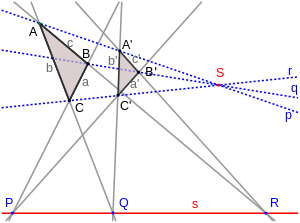
\includegraphics[scale=0.6]{desargues.png}  
\end{center}

\subsubsection{Plan de Hughes}
Jusqu'ici, tous les plans projectifs que nous avons vus étaient des plans desarguesiens : le théorème de Desargues est vérifié sur ces plans.\\
Cependant, sur certains plans projectifs, le théorème de Desargues, c'est le cas des plans de Hughes.\vspace{1\baselineskip}\\

Soit q un nombre premier impair (i.e. différent de 2).\\
Le plan de Hughes se base sur le corps fini $\mathbb{F}_{q^2}$ en utilisant toutefois une multiplication définie différemment de la multiplication ordinaire et non-commutative.\\
On construit $q**2-q+1$ droites d'équation $x + \alpha \circ y + z = 0$ que l'on notera $L(\alpha)$ comme on l'a fait pour la construction des plans projectifs sur des corps finis. On peut ensuite trouver pour chacune un ensemble de $q^2 + q + 1$ droites définies de la façon suivante à partir de n'importe quelle matrice A de taille 3*3 dont les éléments appartiennent à $\mathbb(F)_q$ et telle que $A^{q^2+q+1}=kI$ mais pas pour une puissance plus petite:
\begin{center}
 $ \{A^nL(\alpha) | 0 \leq n \leq q^2 + q\}$
\end{center}
J'ai fait puis ajouté la fonction HughesPlane dans le fichier $block\_design.py$ qui regroupe certaines fonctions comme $projective\_plane$ qui utilise la construction à partir des corps finis faite par la fonction $DesarguesianProjectivePlaneDesign$ aussi dans ce fichier.\\ Cette fonction a été acceptée pour être implémentée dans Sage, ce qui a été fait dans la version beta3 de Sage 6.8 le 4 Juin.
Mon ticket sur le trac de Sage est visible à l'adresse : http://trac.sagemath.org/ticket/18527.\vspace{1\baselineskip}\\
Cette fonction s'appuie sur deux autres fonctions dont une fabrique une matrice A comme expliqué ci-dessus et une autre qui normalise les points ( $(a,b,c)k = (a,b,c)$ ). La fonction principale $HughesPlane$ suit la méthode de construction expliquée précédemment.
\begin{sageverbatim}
 sage: H = designs.HughesPlane(9)
 sage: H
 (91,10,1)-Balanced Incomplete Block Design
\end{sageverbatim}
Les \textit{Balanced Incomplete Block Design} sont des designs combinatoires ou plus précisemment des structures d'incidence avec 3 paramètres, ici $(91, 10, 1)$, ce qui signifie qu'il y a dans cette structure 91 points, 10 points par droite et par deux points passent une droite, ce qui correspond parfaitement à ce que l'on a vu sur les plans projectifs (ici $k=9$ : $k+1=10$ et $k^2+k+1=91$).\\
Nous allons montrer que ce plan de Hughes n'est pas desarguesien. J'ai recherché avec un algorithme les points qui nous permettraient de montrer ceci, je prends donc ici les triangles $(0,1,10)$ et $(57, 70, 59)$. Nous allons montrer que les intersection $D_{0,1} \cap D_{57,70}$, $D_{1,10} \cap D_{70,59}$ et $D_{10,0} \cap D_{59,57}$ sont alignées tandis que les droites $D_{0,70}$, $D_{1,59}$ et $D_{10,57}$ ne s'intersectent pas en un seul point.
\begin{sageverbatim}
 sage: blocks = H.blocks()
 sage: blocks[:3]
 [[0, 1, 2, 3, 4, 5, 6, 7, 8, 81],
 [0, 9, 18, 27, 36, 45, 54, 63, 72, 90],
 [0, 10, 20, 30, 40, 50, 60, 70, 80, 89],
 [0, 11, 23, 31, 43, 51, 55, 71, 75, 88]]
\end{sageverbatim}
La méthode $.blocks()$ depuis une structure d'incidence permet de nous donner une la liste des droites. Il y en a 91 donc je me contente d'en afficher 4.
\begin{sageverbatim}
 line = lambda p,q: (b for b in blocks if p in b and q in b).next()
\end{sageverbatim}
On crée une fonction $line$ qui à p,q associe la droite qui passe par p et q.
\begin{sageverbatim}
 sage: set(line(0, 1)).intersection(line(57, 70))
 {2}
 sage: set(line(1, 10)).intersection(line(70, 59))
 {73}
 sage: set(line(10, 0)).intersection(line(59, 57))
 {60}
\end{sageverbatim}
$line$ nous renvoie une liste (une droite est une liste de points). Nous cherchons à avoir l'intersection de deux listes, ce qui n'est pas possible. Grâce à la fonction $set$, on transforme une des deux listes en un ensemble que l'on peut maintenant utiliser pour trouver l'intersection avec une liste. Nos intersections sont donc les points 2, 73 et 60.
\begin{sageverbatim}
 sage: line(2, 73) == line(73, 60)
 True
\end{sageverbatim}
La droite passant par 2 et 73 est la-même que celle passant par 73 et 60, on a donc bien que les points 2, 60 et 73 sont alignés.
\begin{sageverbatim}
 sage: set(line(0, 57)).intersection(line(1, 70))
 {82}
 sage: set(line(1, 70)).intersection(line(10, 59))
 {72}
\end{sageverbatim}
Les droites $D_{0,70}$, $D_{1,59}$ et $D_{10,57}$ ne sont pas concourrantes.
Plus concrètement voilà ce qu'il se passe dans ce plan de Hughes:
\begin{center}
  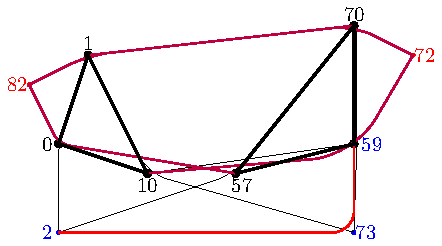
\includegraphics[scale=1.5]{Hughestikz.pdf}
\end{center}
72 et 82 devraient être le même point si le théorème de Desargues s'appliquait ici.






\newpage

\section{Le logiciel Sage}
\subsection{Présentation}
\textit{SageMath} est un logiciel libre de mathématiques qui se veut être une alternative libre à Matlab, Maple...\vspace{1\baselineskip}\\

Il est basé sur le langage Python et combine plusieurs dizaines de programmes libres dans une interface commune.\\
SageMath permet de travailler sur une vaste gamme de Mathématiques. Au cours de ce stage je ne travaille que dans la partie combinatoire de Sage et plus précisemment dans les designs combinatoires.
\vspace{3\baselineskip}
\begin{center}
  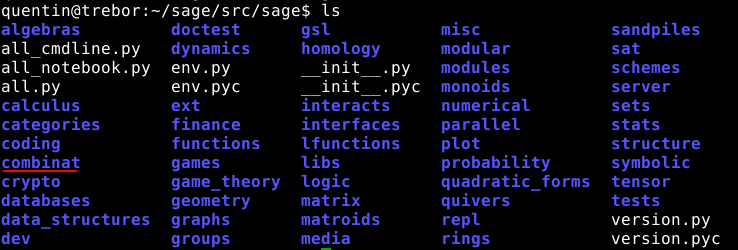
\includegraphics[scale=0.6]{matieres.jpg}
\end{center}
\vspace{3\baselineskip}
Sage étant un logiciel libre, le code source est entièrement accessible et modifiable. Il est en constante évolution, plusieurs mises à jours stables sortent par année. Le développement de Sage (les implémentations de nouvelles fonctions, de nouvelles classes, les corrections de bugs) se fait par tou-te-s les utilisat-rice-teurs qui proposent via le Trac de Sage (application web Open Source de gestion de projets) leur apport qui est ensuite discuté et éventuellement validé.








\newpage
\subsection{La programmation linéaire}
  Un programme linéaire est un système d’équations linéaires dont on cherche une solution optimale. Résoudre un programme linéaire revient à trouver la valeur des variables qui maximise (ou minimise) une fonction objectif, tout en satisfaisant un système de contraintes.
\vspace{1\baselineskip}
\begin{Ex}
  On cherche à maximiser $x + y + 3z$ tel que : \\
  $x + 2y \leq 4$\\
  $5z - y \leq 8$\\
  La solution ici est $x = 4, y = 0, z = 1.6$
\end{Ex}
\vspace{1\baselineskip}
La programmation linéaire lorsqu'on l'utilise est pour nous une boite noire. Le fonctionnement de cette boite est compliqué et bien optimisé. Il nous évite la programmation de grandes boucles très couteuses et bien trop longues dès que l'on a suffisamment de variables. Ces boucles testeraient alors toutes les combinaisons pour chercher celle qui maximise la fonction objectif (et encore, cette méthode n'est pas vraiment possible sur les réels ou les entiers).\\
C'est un outil très utile pour les problèmes combinatoires.
\vspace{1\baselineskip}
\begin{Ex}
  Pour comprendre les problèmes que l'on va chercher à résoudre, nous allons prendre un exemple plus concret:\vspace{1\baselineskip} \\
  On a devant nous notre sac à dos ayant une capacité limitée C que nous devons remplir avec des objets à notre disposition ayant chacun une utilité et un poids propres fixés entre 0 et 1. Par exemple, une gourde aura un poids de 0.39 pour une utilité de 0.85 tandis qu'un livre aura un poids de 0.35 pour une utilité de 0.26 (selon le livre).\vspace{1\baselineskip}\\
  Soit o un objet. On va introduire une variable binaire ``prendre'' telle que $prendre[o]=1$ si on prend o et 0 si on ne le prend pas. \\
  Notre objectif est d'avoir un sac rempli des objets les plus utiles, on veut donc maximiser:
  \begin{center}
    $\sum_o utilit\acute{e}[o] * prendre[o]$
  \end{center}
  Cependant notre sac ayant une capacité limitée, il faut bien ajouter une contrainte sur le poids:
  \begin{center}
    $\sum_o poids[o] * prendre[o] \leq C$
  \end{center}
  Grâce à la programmation linéaire, on pourra donc savoir quelle combinaison d'objets pouvant rentrer dans notre sac est la plus utile.
  \end{Ex}
\newpage
\subsubsection{Dans Sage}
Nous avons dans Sage la classe $MixedIntegerLinearProgram$ qui représente les programmes linéaires que nous avons vu.
Nous allons résoudre le premier exemple avec Sage:
\begin{sageverbatim}
sage: p = MixedIntegerLinearProgram()
sage: x, y, z = p['x'], p['y'], p['z']    # on definit les variables
sage: p.set_objective( x + y + 3*z )
sage: p.add_constraint( x + 2*y <= 4 )
sage: p.add_constraint ( 5*z - y <= 8 )
sage: p.solve()         # sage nous retourne la valeur maximale de l'objectif
8.8
sage: p.get_values(x,y,z)    # on peut demander les valeurs des variables
[4.0, 0.0, 1.6]
\end{sageverbatim}

La programmation linéaire va nous être utile pour trouver les arcs et les blocking set dans les plans projectifs finis. En effet, en associant une valeur binaire à chaque point du plan : 1 si on prend le point dans l'ensemble recherché, 0 sinon.\\
A partir de cet énoncé, on peut faire un programme pour trouver un arc de cardinalité maximale ou un \textit{committee} (un \textit{blocking set} de cardinalité minimale).

Soit s une structure d'incidence :

\begin{lstlisting}
from sage.numerical.mip import MIPSolverException
from sage.categories.sets_cat import EmptySetError
          
def arc(s):   
    p=MixedIntegerLinearProgram()
    b=p.new_variable(binary=True)
# La variable b comme une variable binaire #

    p.set_objective(p.sum(b[v] for v in s._points))
# Notre objectif est le nombre de points dans notre arc #

    for i in s._blocks:
        p.add_constraint(p.sum(b[k] for k in i)<=2)
# On ne doit avoir au maximum que deux points d'un arc sur une ligne #
        
    try:
        p.solve()
        r=p.get_values(b)
        return [i for (i,j) in r.items() if j==1]
    except MIPSolverException:
        raise EmptySetError('There is  no arc in this incidence structure.')
\end{lstlisting}
\newpage
\begin{lstlisting}
def blocking_set(s):
    p=MixedIntegerLinearProgram(maximization=False)
# On minimise plutot que maximise #

    b=p.new_variable(binary=True)
    p.set_objective(p.sum(b[v] for v in s._points))
    for i in s._blocks:
        p.add_constraint(p.sum(b[k] for k in i)>=1)
# Chaque ligne doit etre intersectee #

        p.add_constraint(p.sum(b[k] for k in i)<=len(i)-1)
# Aucune ligne ne doit etre contenue entiere #
        
    try:
        p.solve()
        r=p.get_values(b)
        return [i for (i,j) in r.items() if j==1]
    except MIPSolverException :
        raise EmptySetError('There is no blocking set in this
    incidence structure')  
\end{lstlisting}
\newpage
\thispagestyle{empty}

\section*{Annexes}

\includegraphics[scale=0.43]{dobble1.png}
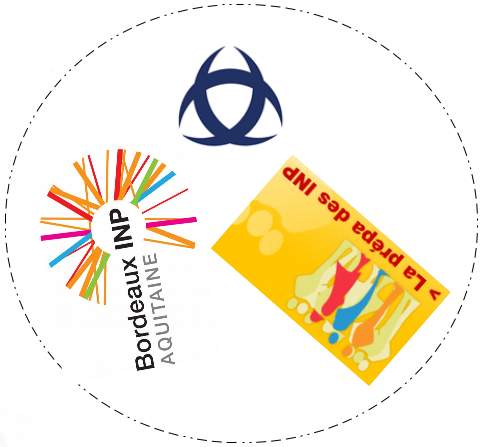
\includegraphics[scale=0.43]{dobble2.png}\\
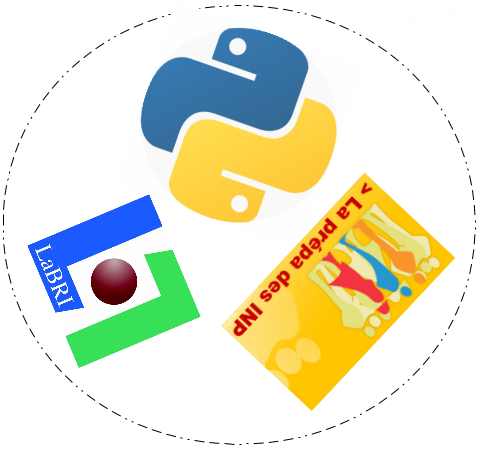
\includegraphics[scale=0.43]{dobble3.png}

\includegraphics[scale=0.43]{dobble4.png}\\
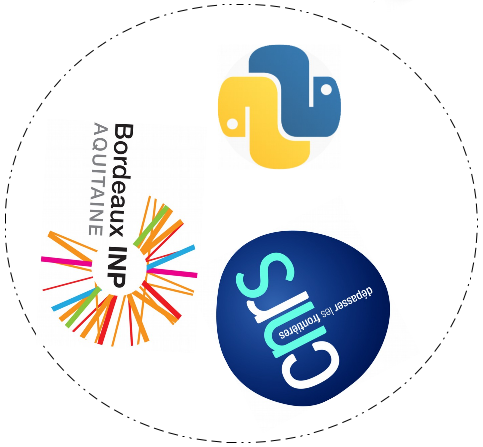
\includegraphics[scale=0.43]{dobble5.png}

\includegraphics[scale=0.43]{dobble6.png}\\

\includegraphics[scale=0.43]{dobble7.png}
\end{document}
